% !TEX program = xelatex
\documentclass[11pt,a4paper]{article}

\usepackage[a4paper,margin=2.3cm,headheight=14pt]{geometry}
\usepackage{fontspec}
\usepackage{amsmath,amssymb}
\usepackage[dvipsnames,table]{xcolor}

% ---------- colours ----------
\definecolor{acnavy}{RGB}{26,54,93}
\definecolor{acgreen}{RGB}{30,110,60}
\definecolor{acamber}{RGB}{214,137,16}
\definecolor{acplum}{RGB}{110,50,140}
\definecolor{acteal}{RGB}{0,120,125}

\usepackage{tikz}
\usetikzlibrary{arrows.meta,positioning,calc,shapes.geometric,fit,backgrounds}
\usepackage[most]{tcolorbox}
\usepackage{booktabs,array,tabularx,multirow}
\usepackage{enumitem}
\usepackage{titlesec}
\usepackage{fancyhdr}
\usepackage{microtype}
\usepackage[colorlinks=true,linkcolor=acnavy,urlcolor=acnavy,citecolor=acnavy,
  pdftitle={Basics of Accounting -- Part 1: Detailed Study Notes},
  pdfsubject={Financial Analysis Course}]{hyperref}

% ---------- rupee symbol (font fallback) ----------
\newfontfamily\rsfont{DejaVu Sans}
\newcommand{\Rs}{{\rsfont ₹}}

% ---------- layout ----------
\setlength{\parindent}{0pt}
\setlength{\parskip}{5pt plus 1pt}
\linespread{1.07}
\setlist{itemsep=2pt,topsep=4pt,parsep=0pt}
\renewcommand{\arraystretch}{1.3}
\newcolumntype{Y}{>{\raggedright\arraybackslash}X}
\setcounter{tocdepth}{2}

\titleformat{\section}{\Large\bfseries\sffamily\color{acnavy}}{\thesection}{0.7em}{}[{\color{acnavy}\titlerule[0.8pt]}]
\titleformat{\subsection}{\large\bfseries\sffamily\color{acnavy!85!black}}{\thesubsection}{0.6em}{}
\titleformat{\subsubsection}{\normalsize\bfseries\sffamily\color{acgreen}}{\thesubsubsection}{0.6em}{}
\titlespacing*{\section}{0pt}{18pt}{8pt}
\titlespacing*{\subsection}{0pt}{12pt}{4pt}
\titlespacing*{\subsubsection}{0pt}{8pt}{2pt}

\pagestyle{fancy}
\fancyhf{}
\fancyhead[L]{\small\sffamily\color{gray}Basics of Accounting --- Part 1}
\fancyhead[R]{\small\sffamily\color{gray}\leftmark}
\fancyfoot[C]{\small\sffamily\thepage}
\renewcommand{\headrulewidth}{0.3pt}

% ---------- coloured boxes ----------
\tcbset{boxstyle/.style={enhanced,breakable,arc=2pt,boxrule=0.6pt,
  left=8pt,right=8pt,top=6pt,bottom=6pt,
  fonttitle=\bfseries\sffamily\small,before skip=8pt,after skip=10pt}}
\newtcolorbox{defbox}[1]{boxstyle,colback=acnavy!5,colframe=acnavy,title={Definition: #1}}
\newtcolorbox{keybox}{boxstyle,colback=acgreen!6,colframe=acgreen,title={Key Idea}}
\newtcolorbox{impbox}[1][Important]{boxstyle,colback=acamber!9,colframe=acamber,title={#1}}
\newtcolorbox{exbox}[1]{boxstyle,colback=acplum!5,colframe=acplum,title={Example: #1}}
\newtcolorbox{casebox}[1]{boxstyle,colback=acteal!6,colframe=acteal,title={Case Study: #1}}
\newtcolorbox{notebox}[1][Note]{boxstyle,colback=gray!8,colframe=gray!70,title={#1}}

% ---------- TikZ styles ----------
\tikzset{
  stage/.style={draw=acnavy,fill=acnavy!10,rounded corners=3pt,minimum width=1.9cm,
    minimum height=1.0cm,align=center,font=\sffamily\scriptsize\bfseries},
  flowbox/.style={draw=acnavy,fill=acnavy!10,rounded corners=3pt,minimum height=0.95cm,
    align=center,font=\sffamily\small\bfseries,inner sep=5pt},
  outbox/.style={draw=acgreen,fill=acgreen!10,rounded corners=3pt,minimum height=0.95cm,
    align=center,font=\sffamily\small\bfseries,inner sep=5pt},
  arr/.style={-{Stealth[length=2mm]},thick,acnavy},
  capt/.style={font=\sffamily\tiny,text width=1.9cm,align=center,text=black!70}
}

\begin{document}

% =====================================================================
%                              TITLE PAGE
% =====================================================================
\begin{titlepage}
\thispagestyle{empty}
\begin{tikzpicture}[remember picture,overlay]
  \fill[acnavy] (current page.north west) rectangle ($(current page.north east)+(0,-12.6cm)$);
  \fill[acamber] ($(current page.north west)+(0,-12.6cm)$) rectangle ($(current page.north east)+(0,-12.9cm)$);
\end{tikzpicture}
\vspace*{1.6cm}
{\color{white}\sffamily
{\large\bfseries FINANCIAL ANALYSIS COURSE \ $\cdot$ \ STUDY NOTES}\\[1.4cm]
{\fontsize{36}{42}\selectfont\bfseries Basics of\\[2pt]Accounting}\\[0.7cm]
{\fontsize{20}{24}\selectfont Part 1: Introduction to Accounting}\\[0.7cm]
{\large Meaning $\cdot$ Functions $\cdot$ Accounting Cycle $\cdot$ Objectives\\
Branches $\cdot$ Limitations $\cdot$ Types of Financial Information}}
\vfill
{\sffamily
\begin{tcolorbox}[enhanced,colback=white,colframe=acnavy!40,boxrule=0.5pt,arc=3pt]
\textbf{What these notes are.} A detailed, explanatory rewrite of the lecture notes on the
\emph{Basics of Accounting} (Parts 1\_A, 1\_B and 1\_C). Every idea in the lecture notes is
covered, in a sequential order, with definitions, rules, formulas, worked examples and
case studies, followed by a glossary and a revision section. They are written so that
a reader with no prior accounting background can follow them from start to finish.
\end{tcolorbox}}
\vspace{0.6cm}
\begin{center}\sffamily\color{gray} October 2026\end{center}
\end{titlepage}

% =====================================================================
%                         ABOUT / HOW TO USE
% =====================================================================
\section*{About These Notes}
\addcontentsline{toc}{section}{About These Notes}
\markboth{About These Notes}{About These Notes}

\subsection*{How the notes are organised}
The notes follow one logical thread: \textbf{why accounting exists} $\rightarrow$
\textbf{what accounting is} $\rightarrow$ \textbf{what it does and how it is organised}
$\rightarrow$ \textbf{what it can and cannot tell us} $\rightarrow$ \textbf{what information it produces}.

\begin{center}
\footnotesize\renewcommand{\arraystretch}{1.08}
\begin{tabularx}{\textwidth}{@{}c Y l@{}}
\toprule
\rowcolor{acnavy!15}\textbf{Section} & \textbf{Topic} & \textbf{Lecture part}\\
\midrule
1 & Why a business needs accounting; business transactions & 1\_A\\
2 & Meaning and definition of accounting & 1\_A\\
3 & Accountancy, bookkeeping and accounting & 1\_B \& 1\_C\\
4 & Luca Pacioli, the ``Father of Accounting'' & 1\_A\\
5 & Objectives and purpose of accounting & 1\_A, 1\_B \& 1\_C\\
6 & Users of accounting information & 1\_A, 1\_B \& 1\_C\\
7 & The seven functions of accounting & 1\_A\\
8 & The accounting cycle & 1\_A\\
9 & Worked case study: from transaction to decision & 1\_A (big picture)\\
10 & Financial, cost and management accounting & 1\_B \& 1\_C\\
11 & Accounting as a science and as an art & 1\_B \& 1\_C\\
12 & Uses and advantages of accounting & 1\_B \& 1\_C\\
13 & Limitations of accounting & 1\_B \& 1\_C\\
14 & Types of accounting information & 1\_B \& 1\_C\\
15 & The complete conceptual framework & 1\_B \& 1\_C\\
16 & Glossary of key terms & all\\
17 & Revision: summaries, common mix-ups, self-test & all\\
\bottomrule
\end{tabularx}
\end{center}

\subsection*{Colour-coded boxes used throughout}
\begingroup\small\tcbset{boxstyle/.append style={before skip=3pt,after skip=3pt,top=2pt,bottom=2pt}}
\begin{defbox}{Blue box}
Formal definitions of terms. Learn these word for word.
\end{defbox}
\begin{keybox}
Green box: the one-line takeaway of a topic, usually the question that the topic answers.
\end{keybox}
\begin{impbox}
Amber box: rules, warnings, limitations and common traps.
\end{impbox}
\begin{exbox}{Purple box}
Worked examples, with numbers, that illustrate a concept.
\end{exbox}
\begin{casebox}{Teal box}
Longer case studies that tie several concepts together.
\end{casebox}

\begin{notebox}[Conventions]
Amounts are in Indian Rupees (\Rs) using the Indian digit grouping (for example \Rs 5,00,000 means
five lakh). Where an example uses figures that are not in the original lecture notes, the
assumptions are stated explicitly so that nothing is hidden.
\end{notebox}
\endgroup

\clearpage
\tableofcontents
\clearpage

% =====================================================================
%                    1. WHY DOES A BUSINESS NEED ACCOUNTING
% =====================================================================
\section{Why Does a Business Need Accounting?}

\subsection{The need for reliable financial information}

The fundamental objective of a business is generally to \textbf{earn profit} and create value.
But to know whether a business is actually performing well, the owner (and every other stakeholder)
needs \textbf{reliable financial information}.

At the end of an accounting period, such as a month, a quarter or a year, a business will want
answers to questions like the following.

\begin{center}
\small
\begin{tabularx}{\textwidth}{@{}Y Y@{}}
\toprule
\rowcolor{acnavy!15}\textbf{Question the business asks} & \textbf{What it is asking about}\\
\midrule
How much profit or loss did the business make? & Profit or loss for the period\\
How much inventory (stock) is currently held? & Inventory / stock\\
What are the business's assets? & Assets (what the business owns)\\
How much does the business owe to outsiders? & Liabilities (what the business owes)\\
How much is owed to the business by customers or others? & Amounts receivable\\
How much has been invested by the owners? & Owner's capital / equity\\
What are the revenues and expenses? & Components of profit or loss\\
What is the overall financial position? & Assets, liabilities and equity taken together\\
\bottomrule
\end{tabularx}
\end{center}

\subsection{Why memory and loose records are not enough}

These questions \textbf{cannot be answered accurately} by looking at individual transactions
in isolation or by trying to remember what happened during the year. A business may carry out
thousands of transactions in a year, and nobody can reliably recall every sale, purchase,
payment and receipt.

Therefore the business must maintain a:

\begin{keybox}
\textbf{Complete and systematic record of every business transaction of a financial nature.}

Accounting is the system through which these transactions are \emph{recorded, organised,
summarised, analysed and communicated}.
\end{keybox}

\subsection{What is a business transaction?}

\begin{defbox}{Business transaction}
A \textbf{business transaction} is an economic event involving the business that can be
\textbf{measured in monetary terms} and has a \textbf{financial effect} on the business.
\end{defbox}

\textbf{Typical examples}

\begin{itemize}
  \item Purchase of goods
  \item Sale of goods
  \item Payment of salaries
  \item Payment of rent
  \item Purchase of machinery
  \item Receipt of cash from customers
  \item Borrowing money from a bank
  \item Repayment of a loan
  \item Payment to suppliers
\end{itemize}

\textbf{The three tests.} An event is recorded as an accounting transaction when it passes
all three of these tests:

\begin{enumerate}
  \item It \textbf{relates to the business}.
  \item It has \textbf{financial consequences} for the business.
  \item It can be \textbf{measured in money}.
\end{enumerate}

\begin{impbox}[Not every event is an accounting transaction]
Not every event involving a business is recorded. Suppose \emph{the manager decides to hire an
employee next month}. This decision by itself does not create a measurable financial
transaction. It becomes a transaction only when the business actually \textbf{pays the
employee's salary}, because at that point there is a financial effect that can be measured
in money.

Accounting therefore primarily records \textbf{financially measurable economic events}.
\end{impbox}

% =====================================================================
%                    2. MEANING OF ACCOUNTING
% =====================================================================
\section{Meaning of Accounting}

\subsection{The definition}

\begin{defbox}{Accounting}
Accounting is the process of \textbf{identifying, recording, classifying, summarising,
interpreting and communicating} financial information of a business to its users for
\textbf{judgement and decision-making}.
\end{defbox}

This definition shows that accounting is \textbf{much more than simply recording transactions}.
It is a sequence of activities:

\[
\boxed{\text{Identify}\rightarrow\text{Record}\rightarrow\text{Classify}\rightarrow\text{Summarise}\rightarrow\text{Analyse}\rightarrow\text{Interpret}\rightarrow\text{Communicate}}
\]

\begin{notebox}[Six verbs or seven?]
The definition above names six activities. In the lecture's list of functions, \emph{analysing}
is shown as a separate seventh activity, sitting between summarising and interpreting. Many
textbook versions of the definition include it. In either case, remember the \textbf{seven
functions}, which are developed in Section~\ref{sec:functions}.
\end{notebox}

\subsection{Reading the definition word by word}

\begin{center}
\small
\begin{tabularx}{\textwidth}{@{}l Y@{}}
\toprule
\rowcolor{acnavy!15}\textbf{Word in the definition} & \textbf{What it means}\\
\midrule
\textbf{Process} & Accounting is a continuing series of steps, not a single act.\\
\textbf{Identifying} & Deciding which events are business transactions with a measurable financial effect.\\
\textbf{Recording} & Entering identified transactions systematically, in chronological order.\\
\textbf{Classifying} & Grouping similar transactions together under suitable accounts.\\
\textbf{Summarising} & Condensing the classified data into compact financial statements.\\
\textbf{Interpreting} & Giving meaning to the numbers and relationships found.\\
\textbf{Communicating} & Delivering the information to those who need it.\\
\textbf{Financial information} & Information measured in money terms.\\
\textbf{Users} & Management, owners, investors, lenders, creditors, government, and others.\\
\textbf{Judgement and decision-making} & The final purpose: users act on the information.\\
\bottomrule
\end{tabularx}
\end{center}

\subsection{Accounting as an information system}

Accounting can be viewed as a system that converts \textbf{raw financial transactions into useful
information}.

\begin{center}
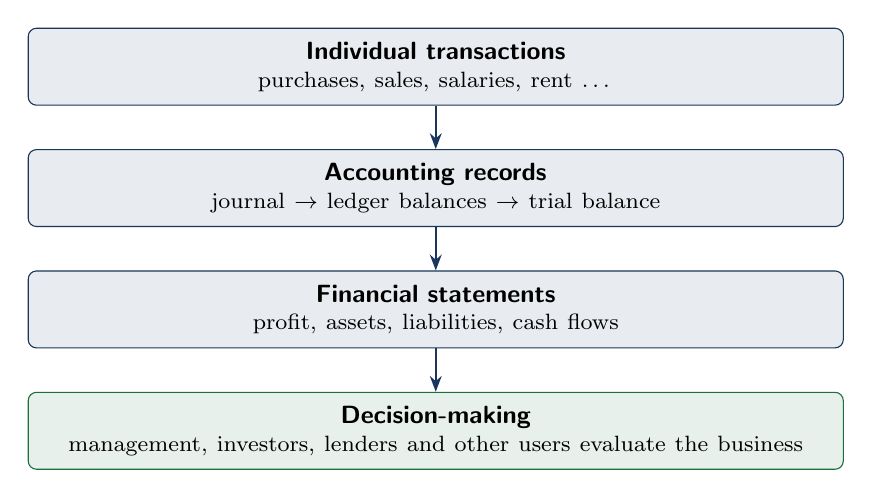
\begin{tikzpicture}[node distance=0.55cm]
  \node[flowbox,text width=10cm] (t) {Individual transactions\\[-1pt]\normalfont\footnotesize purchases, sales, salaries, rent \ldots};
  \node[flowbox,below=of t,text width=10cm] (r) {Accounting records\\[-1pt]\normalfont\footnotesize journal $\rightarrow$ ledger balances $\rightarrow$ trial balance};
  \node[flowbox,below=of r,text width=10cm] (f) {Financial statements\\[-1pt]\normalfont\footnotesize profit, assets, liabilities, cash flows};
  \node[outbox,below=of f,text width=10cm] (d) {Decision-making\\[-1pt]\normalfont\footnotesize management, investors, lenders and other users evaluate the business};
  \draw[arr] (t) -- (r);
  \draw[arr] (r) -- (f);
  \draw[arr] (f) -- (d);
\end{tikzpicture}
\end{center}

\begin{exbox}{From raw transactions to a result}
Suppose a business has these four individual transactions in a period:
\begin{itemize}
  \item Purchase of inventory: \Rs 50,000
  \item Sale of goods: \Rs 80,000
  \item Salary paid: \Rs 10,000
  \item Rent paid: \Rs 5,000
\end{itemize}
Individually these are just four events. After they are recorded, classified and summarised,
the business can see, for example, total sales, total purchases and total expenses, and it
can compute its result. \emph{Assuming all the inventory purchased was sold in the period}:
\[
\text{Profit}=80{,}000-50{,}000-10{,}000-5{,}000=\Rs\,15{,}000 .
\]
Management, lenders or investors can then evaluate the business using such information.
\end{exbox}

% =====================================================================
%               3. ACCOUNTANCY, BOOKKEEPING, ACCOUNTING
% =====================================================================
\section{Accountancy, Bookkeeping and Accounting}

Three similar-sounding words are used in this subject. They are related but different.

\subsection{Accountancy}

\begin{defbox}{Accountancy}
\textbf{Accountancy} is the systematic \textbf{body of knowledge} concerning accounting,
including the \textbf{principles, concepts, rules, conventions, techniques and practices}
that are applied in accounting.
\end{defbox}

In simple terms: \emph{accounting is the practical process of recording and processing financial
information, whereas accountancy is the broader body of knowledge underlying that process.}
Accountancy covers the theoretical and practical framework within which accounting is carried out.

\[
\boxed{\text{Accountancy}=\text{Theory}+\text{Principles}+\text{Concepts}+\text{Practices of Accounting}}
\]

\subsection{Bookkeeping}

\begin{defbox}{Bookkeeping}
\textbf{Bookkeeping} is the process of recording business transactions having monetary aspects
in the books of accounts.
\end{defbox}

Bookkeeping deals primarily with:

\[
\boxed{\text{Bookkeeping}\rightarrow\text{Identify}+\text{Measure}+\text{Record}+\text{Classify}}
\]

\textbf{Nature of bookkeeping.} It is largely routine, clerical, procedural and record-oriented,
and it generally requires less analytical judgement than the later stages of accounting.

\subsection{Accounting (in the narrower, post-bookkeeping sense)}

Accounting is broader than bookkeeping. It begins with the information generated by
bookkeeping and then involves:

\[
\boxed{\text{Accounting}\rightarrow\text{Summarise}+\text{Analyse}+\text{Interpret}+\text{Communicate}}
\]

\begin{keybox}
\textbf{Bookkeeping is a part of accounting.} Bookkeeping provides the basic accounting
records; accounting turns those records into meaningful financial information.
\[
\boxed{\text{Bookkeeping}\subset\text{Accounting}}
\]
\end{keybox}

\subsection{Bookkeeping versus accounting}

\begin{center}
\small
\begin{tabularx}{\textwidth}{@{}l Y Y@{}}
\toprule
\rowcolor{acnavy!15}\textbf{Basis} & \textbf{Bookkeeping} & \textbf{Accounting}\\
\midrule
\textbf{Objective} & To maintain systematic records of transactions of a financial nature & To ascertain the net results and financial position of the business\\
\textbf{Phase} & The recording phase of the accounting system & The summarising phase, and subsequent analysis and interpretation\\
\textbf{Stage} & Primary (initial) stage & Secondary stage, beginning after bookkeeping\\
\textbf{Nature of skills} & Routine and clerical & Analytical; needs accounting knowledge and judgement\\
\textbf{Who performs it} & Bookkeepers / bookkeeping staff & Accountants / accounting staff\\
\bottomrule
\end{tabularx}
\end{center}

\subsection{The overall flow}

\begin{center}
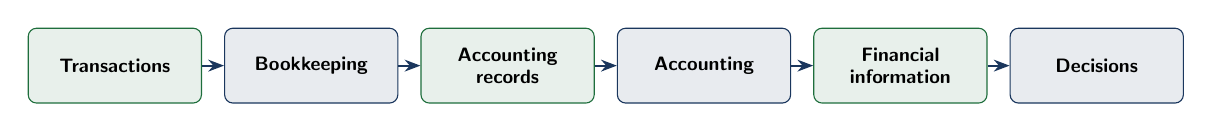
\begin{tikzpicture}[node distance=0.28cm]
  \node[outbox,font=\sffamily\scriptsize\bfseries,minimum width=2.2cm] (a) {Transactions};
  \node[flowbox,font=\sffamily\scriptsize\bfseries,minimum width=2.2cm,right=of a] (b) {Bookkeeping};
  \node[outbox,font=\sffamily\scriptsize\bfseries,minimum width=2.2cm,right=of b] (c) {Accounting\\records};
  \node[flowbox,font=\sffamily\scriptsize\bfseries,minimum width=2.2cm,right=of c] (d) {Accounting};
  \node[outbox,font=\sffamily\scriptsize\bfseries,minimum width=2.2cm,right=of d] (e) {Financial\\information};
  \node[flowbox,font=\sffamily\scriptsize\bfseries,minimum width=2.2cm,right=of e] (f) {Decisions};
  \foreach \x/\y in {a/b,b/c,c/d,d/e,e/f} \draw[arr] (\x) -- (\y);
\end{tikzpicture}
\end{center}

\subsection{Accountancy vs.\ accounting vs.\ bookkeeping on one page}

\begin{center}
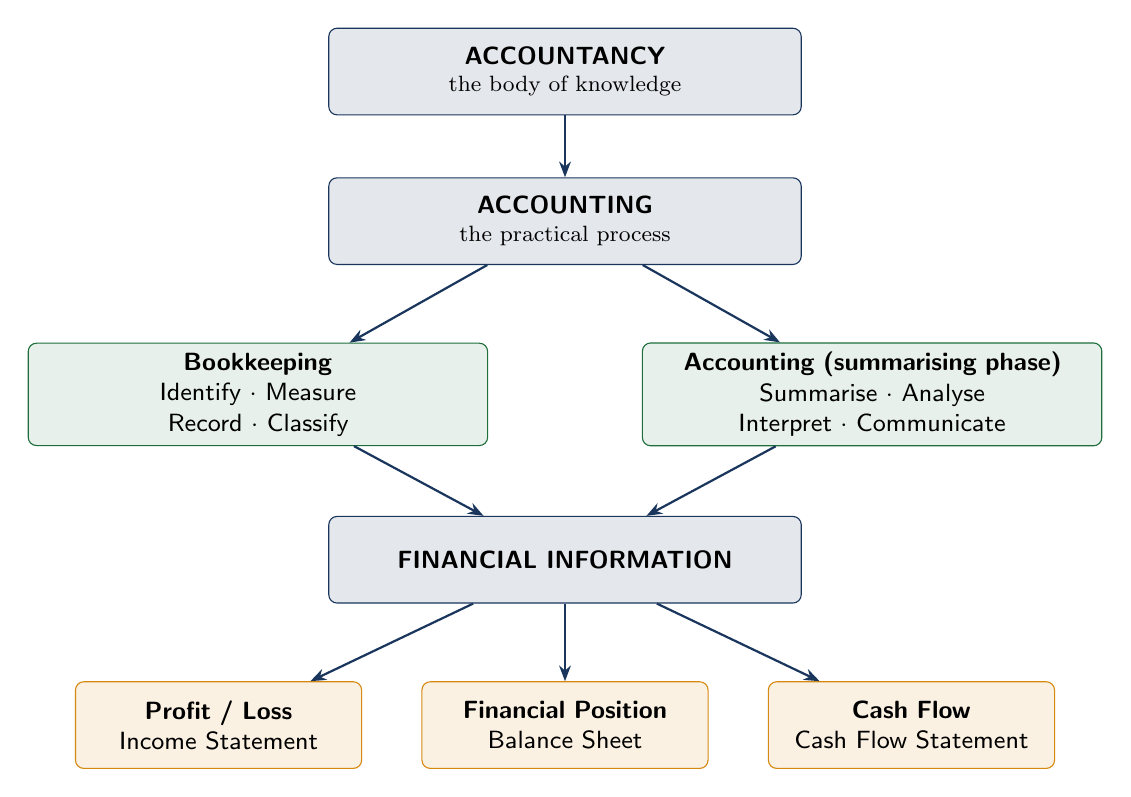
\begin{tikzpicture}[
  big/.style={draw=acnavy,fill=acnavy!12,rounded corners=3pt,align=center,font=\sffamily\small\bfseries,minimum width=6cm,minimum height=1.1cm},
  mid/.style={draw=acgreen,fill=acgreen!10,rounded corners=3pt,align=center,font=\sffamily\small,text width=5.6cm,minimum height=1.3cm},
  info/.style={draw=acamber,fill=acamber!12,rounded corners=3pt,align=center,font=\sffamily\small,text width=3.4cm,minimum height=1.1cm}]
  \node[big] (acy) at (0,0) {ACCOUNTANCY\\[-1pt]\normalfont\footnotesize the body of knowledge};
  \node[big] (acg) at (0,-1.9) {ACCOUNTING\\[-1pt]\normalfont\footnotesize the practical process};
  \node[mid] (bk) at (-3.9,-4.1) {\textbf{Bookkeeping}\\Identify $\cdot$ Measure\\Record $\cdot$ Classify};
  \node[mid] (ac) at (3.9,-4.1) {\textbf{Accounting (summarising phase)}\\Summarise $\cdot$ Analyse\\Interpret $\cdot$ Communicate};
  \node[big] (fi) at (0,-6.2) {FINANCIAL INFORMATION};
  \node[info] (pl) at (-4.4,-8.3) {\textbf{Profit / Loss}\\Income Statement};
  \node[info] (bs) at (0,-8.3) {\textbf{Financial Position}\\Balance Sheet};
  \node[info] (cf) at (4.4,-8.3) {\textbf{Cash Flow}\\Cash Flow Statement};
  \draw[arr] (acy) -- (acg);
  \draw[arr] (acg) -- (bk);
  \draw[arr] (acg) -- (ac);
  \draw[arr] (bk) -- (fi);
  \draw[arr] (ac) -- (fi);
  \draw[arr] (fi) -- (pl);
  \draw[arr] (fi) -- (bs);
  \draw[arr] (fi) -- (cf);
\end{tikzpicture}
\end{center}

% =====================================================================
%                          4. PACIOLI
% =====================================================================
\section{Luca Pacioli: The Father of Accounting}

\textbf{Luca Pacioli} is commonly known as the \textbf{Father of Accounting}, particularly because
of his important role in \textbf{documenting and disseminating the principles of double-entry
bookkeeping}.

\begin{center}
\small
\begin{tabularx}{\textwidth}{@{}l Y@{}}
\toprule
\rowcolor{acnavy!15}\textbf{Fact} & \textbf{Detail}\\
\midrule
Who & Luca Pacioli, an Italian mathematician and Franciscan friar\\
Year & \textbf{1494}\\
Work & \emph{Summa de Arithmetica}, which included a description of the Venetian method of bookkeeping based on double-entry principles\\
Why important & His work helped formalise and spread systematic bookkeeping practices that became foundational to modern accounting\\
\bottomrule
\end{tabularx}
\end{center}

\begin{impbox}[Important distinction]
Pacioli did \textbf{not invent every underlying bookkeeping practice from nothing}. He is
especially remembered for \textbf{documenting and popularising} the double-entry bookkeeping
system. In an examination, the safe statement is: \emph{``Luca Pacioli, Father of Accounting,
documented and popularised double-entry bookkeeping in 1494.''}
\end{impbox}

% =====================================================================
%                          5. OBJECTIVES
% =====================================================================
\section{Objectives and Purpose of Accounting}

The broad purpose of accounting is to provide \textbf{reliable financial information for
decision-making}. This purpose is delivered through four major objectives.

\begin{keybox}
\[
\boxed{
\begin{aligned}
1.&\ \text{Maintain a systematic record of business transactions}\\
2.&\ \text{Determine profit or loss}\\
3.&\ \text{Determine financial position}\\
4.&\ \text{Provide information to interested parties}
\end{aligned}}
\]
\end{keybox}

\subsection{Objective 1: Maintain a systematic record of transactions}

The first objective is to maintain a \textbf{complete and systematic record of business
transactions} according to established accounting rules and procedures.

\textbf{Process.} Transactions are first recorded in the \textbf{journal} or in \textbf{subsidiary
books}, and are then \textbf{posted to the ledger}:

\[
\text{Transaction}\rightarrow\text{Journal / Subsidiary Books}\rightarrow\text{Ledger}
\]

\begin{notebox}[What are subsidiary books?]
Subsidiary books are separate books of original entry kept for frequently occurring types of
transaction (for example, a cash book, a sales book or a purchases book), so that the main
journal is not overloaded.
\end{notebox}

\textbf{Why a complete record matters.} A complete record helps to reduce:
\begin{itemize}
  \item omission of transactions,
  \item loss of information,
  \item fraud or unauthorised manipulation,
  \item dependence on human memory.
\end{itemize}

Imagine a business carrying out thousands of transactions every year. Relying on memory would
make an accurate determination of profit, assets, liabilities, receivables and expenses
impossible. Accounting creates a \textbf{permanent and organised record}.

\subsection{Objective 2: Calculate profit or loss}

The second objective is to ascertain the \textbf{net profit earned or net loss suffered during
a particular accounting period}, by considering the business's revenues and expenses.

\[
\boxed{\text{Profit}=\text{Revenue}-\text{Expenses}}\quad(\text{when revenue exceeds expenses})
\]
\[
\boxed{\text{Loss}=\text{Expenses}-\text{Revenue}}\quad(\text{when expenses exceed revenue})
\]

The \textbf{Income Statement / Profit and Loss Account} is prepared to determine the result.

\begin{impbox}[Profit and loss relate to a period of time]
The result always relates to a \textbf{period}, such as one month, one quarter or one financial
year (for example, ``profit for the year ended 31 March 2026'').
\end{impbox}

\subsection{Objective 3: Ascertain the financial position}

Profit alone does not tell the complete story. A business may have earned a profit and still
have substantial liabilities or insufficient resources. Accounting therefore also aims to
determine the \textbf{financial position} of the business, presented in the
\textbf{Balance Sheet / Statement of Financial Position}.

The balance sheet reports three things:

\begin{center}
\small
\begin{tabularx}{\textwidth}{@{}l Y@{}}
\toprule
\rowcolor{acnavy!15}\textbf{Element} & \textbf{Meaning}\\
\midrule
\textbf{Assets} & Resources controlled by the business (what it \emph{owns})\\
\textbf{Liabilities} & Obligations owed by the business to outsiders (what it \emph{owes})\\
\textbf{Capital / Equity} & The owners' residual interest in the business\\
\bottomrule
\end{tabularx}
\end{center}

\subsubsection{The accounting equation}

\[
\boxed{\text{Assets}=\text{Liabilities}+\text{Equity}}
\]

\begin{center}
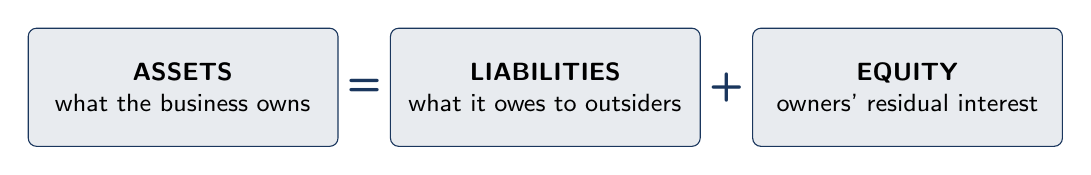
\begin{tikzpicture}[
  eqbox/.style={draw=acnavy,fill=acnavy!10,rounded corners=3pt,align=center,font=\sffamily\small,text width=3.7cm,minimum height=1.5cm},
  sym/.style={font=\sffamily\Large\bfseries,text=acnavy}]
  \node[eqbox] (a) at (0,0) {\textbf{ASSETS}\\what the business owns};
  \node[sym] at (2.3,0) {=};
  \node[eqbox] (l) at (4.6,0) {\textbf{LIABILITIES}\\what it owes to outsiders};
  \node[sym] at (6.9,0) {+};
  \node[eqbox] (e) at (9.2,0) {\textbf{EQUITY}\\owners' residual interest};
\end{tikzpicture}
\end{center}

Rearranging gives the \emph{residual} view of equity:
$\text{Equity}=\text{Assets}-\text{Liabilities}$. The equation is the foundation of everything
that follows, because every transaction must leave it in balance.

\begin{exbox}{How transactions keep the equation in balance}
\begin{center}
\small
\begin{tabularx}{\textwidth}{@{}Y r r r@{}}
\toprule
\rowcolor{acnavy!15}\textbf{Transaction} & \textbf{Assets (\Rs)} & \textbf{Liabilities (\Rs)} & \textbf{Equity (\Rs)}\\
\midrule
1. Owner invests \Rs 1,00,000 in cash & 1,00,000 & 0 & 1,00,000\\
2. Goods bought for \Rs 30,000 cash (cash $\downarrow$, inventory $\uparrow$) & 1,00,000 & 0 & 1,00,000\\
3. Bank loan of \Rs 50,000 received in cash & 1,50,000 & 50,000 & 1,00,000\\
\bottomrule
\end{tabularx}
\end{center}
(Figures are running totals after each transaction.) After each step,
Assets $=$ Liabilities $+$ Equity. In step~2 only the \emph{composition} of assets changes
(cash becomes inventory); in step~3 an asset and a liability rise together.
\end{exbox}

\subsubsection{Income statement versus balance sheet}

\begin{center}
\small
\begin{tabularx}{\textwidth}{@{}l Y Y@{}}
\toprule
\rowcolor{acnavy!15} & \textbf{Income Statement} & \textbf{Balance Sheet}\\
\midrule
\textbf{Question answered} & What happened during the period? & What is the financial position at a particular date?\\
\textbf{Time perspective} & A period of time & A point in time\\
\textbf{Description} & Performance report & A ``screen picture'' (snapshot) of the financial position\\
\bottomrule
\end{tabularx}
\end{center}

\subsection{Objective 4: Provide information to various parties}

Accounting aims to provide financial information to \textbf{interested parties}: owners,
management, creditors, banks and lenders, government authorities, investors and other
stakeholders. This information lets users take appropriate economic decisions, so accounting
is ultimately an \textbf{information and decision-support function}.

\subsection{Other practical purposes (Part 1\_A view)}

Besides the four headline objectives, the lecture lists specific things accounting helps a
business to determine.

\subsubsection{Track inventory (stock)}
Accounting helps determine how much inventory the business holds, how much has been
purchased, how much has been sold and, depending on the accounting system, the value of
closing inventory. This is particularly important for businesses dealing in physical goods.

\subsubsection{Track amounts owed by and to the business}
\begin{itemize}
  \item \textbf{Amounts receivable:} money that customers or other parties owe the business.
  \item \textbf{Amounts payable:} money the business owes suppliers, lenders, employees,
        governments or other parties.
\end{itemize}

\subsubsection{Support decision-making}
Accounting is not merely a historical record-keeping exercise. It is also a
\textbf{decision-support system}. Different users take different decisions, as the next
section shows.

% =====================================================================
%                          6. USERS
% =====================================================================
\section{Users of Accounting Information}

The final accounting function is communication to interested parties. They fall into two groups.

\begin{center}
\small
\begin{tabularx}{\textwidth}{@{}l Y Y@{}}
\toprule
\rowcolor{acnavy!15}\textbf{Group} & \textbf{Users} & \textbf{How they use the information}\\
\midrule
\multirow{3}{*}{\textbf{Internal users}} & Management & Plan and control operations\\
 & Owners & Evaluate profitability\\
 & Other internal decision-makers & Make operating and financing decisions\\
\midrule
\multirow{5}{*}{\textbf{External users}} & Investors / shareholders & Assess performance and prospects\\
 & Banks and lenders & Assess repayment ability\\
 & Creditors & Judge whether dues will be paid\\
 & Government / regulatory authorities & Compliance, taxation and regulation\\
 & Other interested stakeholders & Understand the financial condition of the business\\
\bottomrule
\end{tabularx}
\end{center}

The information reaches users primarily through \textbf{financial reports and statements},
together with other relevant reports.

\begin{notebox}[A note on the table]
The lecture names the user groups and gives the uses for managers, investors, lenders and
owners. The remaining ``how they use it'' entries (creditors, government, other internal
decision-makers) are the natural extensions of the same idea.
\end{notebox}

% =====================================================================
%                          7. FUNCTIONS
% =====================================================================
\section{The Seven Functions of Accounting}
\label{sec:functions}

The lecture identifies \textbf{seven major functions} (processes) of accounting. They are the
stages through which raw business transactions are converted into useful financial
information.

\begin{center}
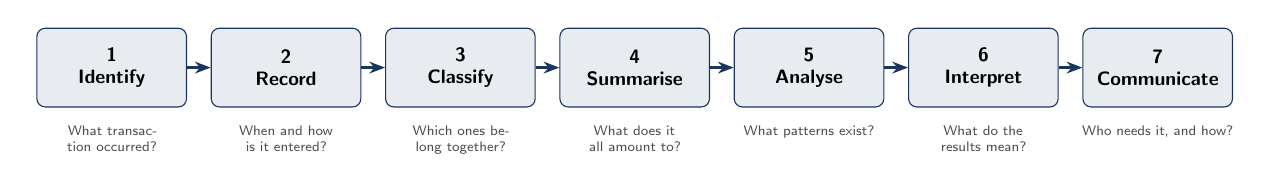
\begin{tikzpicture}[node distance=0.3cm]
  \node[stage] (s1) {1\\Identify};
  \node[stage,right=of s1] (s2) {2\\Record};
  \node[stage,right=of s2] (s3) {3\\Classify};
  \node[stage,right=of s3] (s4) {4\\Summarise};
  \node[stage,right=of s4] (s5) {5\\Analyse};
  \node[stage,right=of s5] (s6) {6\\Interpret};
  \node[stage,right=of s6] (s7) {7\\Communicate};
  \foreach \x/\y in {s1/s2,s2/s3,s3/s4,s4/s5,s5/s6,s6/s7} \draw[arr] (\x) -- (\y);
  \node[capt,below=3pt of s1] {What transaction occurred?};
  \node[capt,below=3pt of s2] {When and how is it entered?};
  \node[capt,below=3pt of s3] {Which ones belong together?};
  \node[capt,below=3pt of s4] {What does it all amount to?};
  \node[capt,below=3pt of s5] {What patterns exist?};
  \node[capt,below=3pt of s6] {What do the results mean?};
  \node[capt,below=3pt of s7] {Who needs it, and how?};
\end{tikzpicture}
\end{center}

\textbf{Memory aid.} Identify $\rightarrow$ Record $\rightarrow$ Group $\rightarrow$ Summarise
$\rightarrow$ Analyse $\rightarrow$ Explain $\rightarrow$ Communicate, or the initials
\textbf{I--R--C--S--A--I--C}.

The important idea is that accounting starts with \textbf{raw financial events} and ends with
\textbf{useful information for decision-making}.

% ---------------------------------------------------------------------
\subsection{Function 1: Identifying}

\textbf{Meaning.} The first function is to \textbf{identify business transactions of a financial
character}. The accountant decides which events (1) relate to the business, and (2) have a
financial effect that can be measured in money.

\textbf{Source documents.} Transactions are identified using documents such as:

\begin{itemize}
  \item Invoices
  \item Agreements / contracts
  \item Cash memos
  \item Receipts
  \item Bills
  \item Bank documents
  \item Purchase orders and other supporting records
\end{itemize}

\begin{exbox}{Identifying a machinery purchase}
A business purchases machinery for \Rs 2,00,000. The invoice or other documentation is the
evidence. The accountant identifies that (i) the business acquired an \textbf{asset},
(ii) the transaction has a monetary value of \Rs 2,00,000, and (iii) it therefore needs to
be recorded.
\end{exbox}

\begin{keybox}
\textbf{Identification answers: ``What financial transaction has occurred?''}
\end{keybox}

% ---------------------------------------------------------------------
\subsection{Function 2: Recording}

Once identified, a transaction must be \textbf{systematically recorded}, generally in
\textbf{chronological order} (the sequence in which transactions occur). The primary record is the
\textbf{journal}, together with subsidiary books where applicable.

\begin{exbox}{Chronological recording}
\begin{itemize}
  \item 1 January: owner invests \Rs 1,00,000.
  \item 3 January: goods purchased for \Rs 30,000.
  \item 5 January: goods sold for \Rs 20,000.
\end{itemize}
They are recorded in exactly this order. Assuming all three are cash transactions, the journal
entries would be:
\begin{center}
\small
\begin{tabular}{@{}l l r r@{}}
\toprule
\rowcolor{acplum!12}\textbf{Date} & \textbf{Account} & \textbf{Debit (\Rs)} & \textbf{Credit (\Rs)}\\
\midrule
1 Jan & Cash A/c \hfill (Dr) & 1,00,000 & \\
      & \quad Capital A/c \hfill (Cr) & & 1,00,000\\
\midrule
3 Jan & Purchases A/c \hfill (Dr) & 30,000 & \\
      & \quad Cash A/c \hfill (Cr) & & 30,000\\
\midrule
5 Jan & Cash A/c \hfill (Dr) & 20,000 & \\
      & \quad Sales A/c \hfill (Cr) & & 20,000\\
\bottomrule
\end{tabular}
\end{center}
\end{exbox}

\subsubsection{The double-entry principle}

Under \textbf{double-entry bookkeeping}, every transaction is recorded through corresponding
\textbf{debits and credits}. For every journal entry:

\[
\boxed{\text{Total Debits}=\text{Total Credits}}
\]

This equality is essential for maintaining the accounting equation, and it provides an
\textbf{internal check} on the recording process.

\begin{keybox}
\textbf{Recording answers: ``When and how should the transaction be entered into the accounting
records?''}
\end{keybox}

% ---------------------------------------------------------------------
\subsection{Function 3: Classifying}

Recording transactions chronologically is not enough. Similar transactions must be
\textbf{grouped together}. This is \textbf{classification}, and it takes place through
\textbf{ledger accounts}.

\begin{exbox}{Why classification is needed}
During the year a business makes 50 cash sales, 20 credit sales, 15 purchases and 12 salary
payments. Instead of re-reading all 97 transactions each time, related transactions are
accumulated in accounts such as:
\begin{itemize}
  \item Sales Account
  \item Purchases Account
  \item Cash Account
  \item Salary Account
  \item Debtors / Receivables Account
  \item Creditors / Payables Account
\end{itemize}
To find the total salary expense, we simply look at the \textbf{Salary Account} instead of
searching through hundreds of transactions.
\end{exbox}

After the ledger accounts are prepared, a \textbf{trial balance} can be drawn up to check the
arithmetical equality of debit and credit balances (Section~\ref{sec:cycle}).

\begin{keybox}
\textbf{Classification answers: ``Which transactions belong together?''}
\end{keybox}

% ---------------------------------------------------------------------
\subsection{Function 4: Summarising}

Accounting records can contain hundreds, thousands or millions of transactions. Decision-makers
do not want to inspect each one. The classified information from the ledger and trial balance
is therefore \textbf{summarised} into financial statements:

\begin{itemize}
  \item \textbf{Income Statement / Profit and Loss Account}
  \item \textbf{Balance Sheet / Statement of Financial Position}
  \item \textbf{Cash Flow Statement}
\end{itemize}

\begin{exbox}{Summarising in practice}
Instead of listing every salary payment separately, the statements show a single line:
\textbf{Salary expense $=$ \Rs 6,50,000}. Instead of listing every asset purchase, the balance
sheet shows the relevant asset balances.
\end{exbox}

\begin{keybox}
\textbf{Summarising answers: ``What does all the recorded information amount to?''}
\end{keybox}

% ---------------------------------------------------------------------
\subsection{Function 5: Analysing}

Once summarised, the information must be \textbf{analysed}. Analysis examines relationships
among financial statement items to understand the business's performance and position. It helps
identify the \textbf{financial strengths} and \textbf{financial weaknesses} of the business.

The main techniques (developed later in financial analysis) are \textbf{ratio analysis},
\textbf{trend analysis} and \textbf{comparative analysis}.

\begin{exbox}{Why one number is not enough}
Suppose a company's sales are increasing, its profit margin is falling, its debt is
increasing and its cash flow is deteriorating. Looking at any single figure (for instance, rising
sales) would give a misleading, rosy picture. Analysis establishes the \textbf{relationships
between items} and shows what the numbers imply together.
\end{exbox}

\begin{keybox}
\textbf{Analysis answers: ``What relationships and patterns exist in the financial information?''}
\end{keybox}

% ---------------------------------------------------------------------
\subsection{Function 6: Interpreting}

Analysis produces relationships and patterns. \textbf{Interpretation} gives them \textbf{meaning}.

\begin{exbox}{Debt-to-equity ratio}
Analysis shows that the \emph{Debt-to-Equity Ratio} has increased significantly. The
\emph{interpretation} is that the company is becoming more dependent on debt financing,
potentially increasing its financial risk.
\end{exbox}

\begin{center}
\small
\begin{tabularx}{\textwidth}{@{}l Y@{}}
\toprule
\rowcolor{acnavy!15}\textbf{Stage} & \textbf{Role}\\
\midrule
\textbf{Analysis} & Identifies the numerical relationship\\
\textbf{Interpretation} & Explains what that relationship means\\
\bottomrule
\end{tabularx}
\end{center}

\begin{keybox}
\textbf{Interpretation answers: ``What do the results of the analysis actually mean?''}
\end{keybox}

% ---------------------------------------------------------------------
\subsection{Function 7: Communicating}

The final function is to \textbf{communicate} the summarised, analysed and interpreted
information to the relevant users (see Section~6 for the full list of internal and external
users). Communication takes place primarily through financial reports and statements, along
with other relevant reports.

\begin{keybox}
\textbf{Communication answers: ``Who needs this information, and how should it be provided to them?''}
\end{keybox}

\subsection{Summary of the seven functions}

\begin{center}
\small
\begin{tabularx}{\textwidth}{@{}c l Y Y@{}}
\toprule
\rowcolor{acnavy!15}\textbf{\#} & \textbf{Function} & \textbf{Core activity} & \textbf{Key question}\\
\midrule
1 & Identifying & Pick out financial transactions using source documents & What transaction occurred?\\
2 & Recording & Enter in the journal, chronologically, by debit and credit & When and how is it entered?\\
3 & Classifying & Group in ledger accounts & Which belong together?\\
4 & Summarising & Prepare trial balance and financial statements & What does it amount to?\\
5 & Analysing & Study relationships among statement items & What patterns exist?\\
6 & Interpreting & Give meaning to the analysis & What does it mean?\\
7 & Communicating & Report to internal and external users & Who needs it, and how?\\
\bottomrule
\end{tabularx}
\end{center}

% =====================================================================
%                          8. ACCOUNTING CYCLE
% =====================================================================
\section{The Accounting Cycle}
\label{sec:cycle}

\subsection{Meaning}

\begin{defbox}{Accounting cycle}
The \textbf{accounting cycle} is the systematic process followed to record and process a
company's financial transactions, beginning when a transaction occurs and ultimately resulting
in the preparation of financial statements and the closing of the accounts.
\end{defbox}

It is called a \textbf{cycle} because the process is \textbf{repeated for each accounting
period}. The simplified version in the lecture is:

\[
\boxed{\begin{aligned}&\text{Financial Transaction}\rightarrow\text{General Journal}\rightarrow\text{General Ledger}\\&\qquad\rightarrow\text{Trial Balance}\rightarrow\text{Financial Statements}\end{aligned}}
\]

\begin{center}
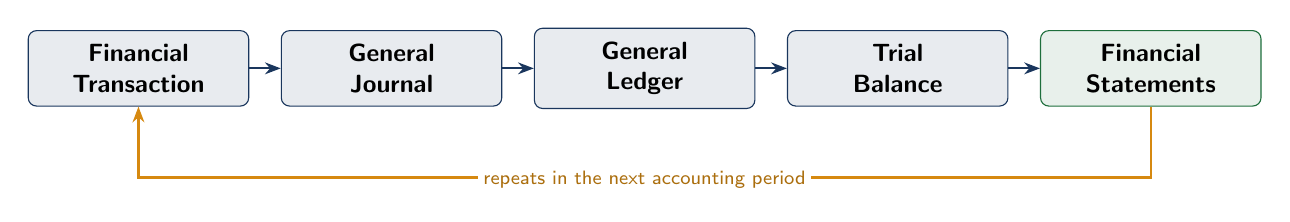
\begin{tikzpicture}[node distance=0.4cm]
  \node[flowbox,minimum width=2.8cm,font=\sffamily\small\bfseries] (n1) {Financial\\Transaction};
  \node[flowbox,minimum width=2.8cm,right=of n1] (n2) {General\\Journal};
  \node[flowbox,minimum width=2.8cm,right=of n2] (n3) {General\\Ledger};
  \node[flowbox,minimum width=2.8cm,right=of n3] (n4) {Trial\\Balance};
  \node[outbox,minimum width=2.8cm,right=of n4] (n5) {Financial\\Statements};
  \foreach \x/\y in {n1/n2,n2/n3,n3/n4,n4/n5} \draw[arr] (\x) -- (\y);
  \draw[arr,acamber] (n5.south) -- ++(0,-0.9) -| (n1.south);
  \node[font=\sffamily\scriptsize,text=acamber!80!black,fill=white,inner sep=2pt] at ($(n3.south)+(0,-0.9)$) {repeats in the next accounting period};
\end{tikzpicture}
\end{center}

\subsection{Stage 1: Financial transactions}

The cycle begins when a \textbf{financial transaction} occurs: a purchase, a sale, payment of
expenses, receipt of cash, purchase of an asset, borrowing money, repayment of debt. The
transaction must first be \textbf{identified and measured in monetary terms}.

\begin{exbox}{Equipment purchase}
A business purchases equipment for \Rs 1,00,000. This is a financial transaction because it
(i) relates to the business, (ii) has financial consequences, and (iii) can be measured in money.
\end{exbox}

\subsection{Stage 2: General journal}

The identified transaction is recorded in the \textbf{journal}, in \textbf{chronological order}.
A journal entry normally specifies:

\begin{itemize}
  \item the accounts affected,
  \item the debit(s) and the credit(s),
  \item the amount,
  \item an explanation (\emph{narration}) where required.
\end{itemize}

\begin{exbox}{Journal entry for the equipment purchase (cash)}
\begin{center}
\begin{tabular}{@{}l r r@{}}
\toprule
\rowcolor{acplum!12}\textbf{Account} & \textbf{Debit} & \textbf{Credit}\\
\midrule
Equipment A/c & \Rs 1,00,000 & ---\\
\quad Cash A/c & --- & \Rs 1,00,000\\
\bottomrule
\end{tabular}
\end{center}
The fundamental requirement is $\boxed{\text{Debit}=\text{Credit}}$.
\end{exbox}

\subsection{Stage 3: Posting to the general ledger}

Journal entries are then \textbf{posted to the General Ledger (GL)}. A ledger contains
\textbf{individual accounts} in which all transactions relating to the same account are
accumulated. All transactions affecting Cash are brought together in the Cash Account; all
transactions affecting Equipment are brought together in the Equipment Account.

The ledger thus transforms the \emph{chronological} information of the journal into an
\emph{account-wise} classification.

\begin{exbox}{The equipment purchase after posting}
\begin{center}
\small
\begin{tabular}{@{}p{3.5cm}|p{3.5cm}@{\hspace{0.8cm}}p{3.5cm}|p{3.5cm}@{}}
\multicolumn{2}{c}{\textbf{Equipment A/c}} & \multicolumn{2}{c}{\textbf{Cash A/c}}\\
\hline
\textbf{Debit} & \textbf{Credit} & \textbf{Debit} & \textbf{Credit}\\
\hline
To Cash \Rs 1,00,000 & & & By Equipment \Rs 1,00,000\\
\hline
\end{tabular}
\end{center}
(The Cash A/c would also carry its other entries, such as the owner's capital introduced;
only the entry for this transaction is shown.)
\end{exbox}

\subsubsection{Journal versus ledger}

\begin{center}
\small
\begin{tabularx}{\textwidth}{@{}Y Y@{}}
\toprule
\rowcolor{acnavy!15}\textbf{Journal} & \textbf{Ledger}\\
\midrule
Records transactions \textbf{chronologically} & Groups transactions \textbf{account-wise}\\
The first formal recording & Classification of recorded transactions\\
Answers ``when did it occur?'' & Helps determine ``what is the balance or effect of this account?''\\
\bottomrule
\end{tabularx}
\end{center}

\subsection{Stage 4: Trial balance}

At the end of an accounting period, the \textbf{balances of the ledger accounts} are listed in a
\textbf{trial balance}. Its basic purpose is to check the \textbf{arithmetical accuracy} of the
records. Ideally:

\[
\boxed{\text{Total Debit Balances}=\text{Total Credit Balances}}
\]

\begin{impbox}[Limitation: an agreeing trial balance is a check, not proof]
A trial balance that agrees does \textbf{not} necessarily mean every accounting error is
absent. Certain errors leave debits equal to credits. Illustrations:
\begin{itemize}
  \item a transaction that was \textbf{completely omitted} (no debit and no credit was posted);
  \item a correct amount posted to the \textbf{wrong account} (for example, to the wrong
        expense account);
  \item two \textbf{offsetting errors} that cancel each other.
\end{itemize}
The trial balance is an important check, but not proof that the accounting records are
completely error-free.
\end{impbox}

\subsection{Stage 5: Financial statements}

After the necessary \textbf{adjustments} and finalisation of account balances, the financial
statements are prepared.

\subsubsection{Income Statement / Profit and Loss Account}
Shows financial performance over a \textbf{period}. It determines whether the business made a
\textbf{profit} or a \textbf{loss}.

\subsubsection{Balance Sheet / Statement of Financial Position}
Shows the financial position at a \textbf{particular point in time}:
$\text{Assets}=\text{Liabilities}+\text{Equity}$.

\subsubsection{Cash Flow Statement}
Shows how cash and cash equivalents changed during a period through different types of cash
flows, broadly classified into:

\begin{center}
\small
\begin{tabularx}{\textwidth}{@{}l Y@{}}
\toprule
\rowcolor{acnavy!15}\textbf{Category} & \textbf{Nature}\\
\midrule
\textbf{Operating activities} & Cash flows from the business's day-to-day operations\\
\textbf{Investing activities} & Cash flows from buying or selling long-term assets and similar investments\\
\textbf{Financing activities} & Cash flows from raising or repaying capital and borrowings\\
\bottomrule
\end{tabularx}
\end{center}

This statement matters because \textbf{profit and cash are not the same thing}.

\subsection{Closing and the next period}

After the statements are prepared, the accounts are closed for the period and the cycle starts
again with the transactions of the next accounting period.

\subsection{Accounting cycle versus functions of accounting}

The two ideas are closely related but should not be confused.

\begin{center}
\small
\begin{tabularx}{\textwidth}{@{}l Y Y@{}}
\toprule
\rowcolor{acnavy!15} & \textbf{Functions of accounting} & \textbf{Accounting cycle}\\
\midrule
\textbf{Focus} & \emph{What accounting does} & The \emph{sequence of procedures} through which records are processed\\
\textbf{Sequence} & Identify $\rightarrow$ Record $\rightarrow$ Classify $\rightarrow$ Summarise $\rightarrow$ Analyse $\rightarrow$ Interpret $\rightarrow$ Communicate & Transaction $\rightarrow$ Journal $\rightarrow$ Ledger $\rightarrow$ Trial Balance $\rightarrow$ Financial Statements $\rightarrow$ Closing / next period\\
\bottomrule
\end{tabularx}
\end{center}

The cycle is the \textbf{operational flow}. The functions describe the \textbf{purpose} of each part of it.

\begin{center}
\small
\begin{tabularx}{\textwidth}{@{}Y Y@{}}
\toprule
\rowcolor{acnavy!15}\textbf{Function} & \textbf{Where it appears in the cycle}\\
\midrule
Identify & Stage 1: the financial transaction is identified and measured\\
Record & Stage 2: general journal\\
Classify & Stage 3: posting to the general ledger\\
Summarise & Stages 4 and 5: trial balance and financial statements\\
Analyse, Interpret, Communicate & Use of the financial statements, after the cycle's outputs are ready\\
\bottomrule
\end{tabularx}
\end{center}

% =====================================================================
%                9. WORKED CASE STUDY
% =====================================================================
\section{Worked Case Study: From Transaction to Decision}

The lecture's ``big picture'' example takes a business that
(i) invests \Rs 5,00,000 capital, (ii) purchases inventory for \Rs 2,00,000, (iii) sells goods
for \Rs 3,00,000, (iv) pays salary of \Rs 40,000 and (v) pays rent of \Rs 20,000.
Initially these are just individual transactions. Below, the full chain of seven functions is
carried out on them.

\begin{notebox}[Assumptions added for the walk-through]
The lecture gives only the five amounts. To complete the numbers we assume that
(a) all five transactions are settled in \textbf{cash}, and (b) \textbf{all inventory purchased is
sold} in the period (so closing inventory is nil). A second scenario at the end relaxes (a).
\end{notebox}

\subsection{Step 1: Identify}
All five events relate to the business, have financial effects and are measurable in money, so
all five are accounting transactions.

\subsection{Step 2: Record (journal)}

\begin{center}
\small
\begin{tabular}{@{}c l r r@{}}
\toprule
\rowcolor{acteal!15}\textbf{No.} & \textbf{Account} & \textbf{Debit (\Rs)} & \textbf{Credit (\Rs)}\\
\midrule
1 & Cash A/c \hfill (Dr) & 5,00,000 & \\
  & \quad Capital A/c \hfill (Cr) & & 5,00,000\\
\midrule
2 & Purchases A/c \hfill (Dr) & 2,00,000 & \\
  & \quad Cash A/c \hfill (Cr) & & 2,00,000\\
\midrule
3 & Cash A/c \hfill (Dr) & 3,00,000 & \\
  & \quad Sales A/c \hfill (Cr) & & 3,00,000\\
\midrule
4 & Salary A/c \hfill (Dr) & 40,000 & \\
  & \quad Cash A/c \hfill (Cr) & & 40,000\\
\midrule
5 & Rent A/c \hfill (Dr) & 20,000 & \\
  & \quad Cash A/c \hfill (Cr) & & 20,000\\
\bottomrule
\end{tabular}
\end{center}

\subsection{Step 3: Classify (ledger)}

Each account collects its own entries. The Cash Account, for instance, becomes:

\begin{center}
\small
\begin{tabular}{@{}p{2.6cm} r | p{2.6cm} r@{}}
\multicolumn{4}{c}{\textbf{Cash A/c}}\\
\hline
\textbf{Debit} & \textbf{\Rs} & \textbf{Credit} & \textbf{\Rs}\\
\hline
Capital & 5,00,000 & Purchases & 2,00,000\\
Sales & 3,00,000 & Salary & 40,000\\
 & & Rent & 20,000\\
 & & \textbf{Balance c/d} & \textbf{5,40,000}\\
\hline
\textbf{Total} & \textbf{8,00,000} & \textbf{Total} & \textbf{8,00,000}\\
\hline
\end{tabular}
\end{center}

The balance of \Rs 5,40,000 is a \textbf{debit balance} (the business has that much cash).

\subsection{Step 4: Summarise}

\textbf{Trial balance}

\begin{center}
\small
\begin{tabular}{@{}l r r@{}}
\toprule
\rowcolor{acteal!15}\textbf{Account} & \textbf{Debit (\Rs)} & \textbf{Credit (\Rs)}\\
\midrule
Cash & 5,40,000 & \\
Purchases & 2,00,000 & \\
Salary & 40,000 & \\
Rent & 20,000 & \\
Capital & & 5,00,000\\
Sales & & 3,00,000\\
\midrule
\textbf{Total} & \textbf{8,00,000} & \textbf{8,00,000}\\
\bottomrule
\end{tabular}
\end{center}

Debits equal credits, so the records are arithmetically consistent.

\textbf{Income statement (for the period)}

\begin{center}
\small
\begin{tabular}{@{}l r r@{}}
\toprule
\rowcolor{acteal!15}\textbf{Particulars} & \textbf{\Rs} & \textbf{\Rs}\\
\midrule
Sales & & 3,00,000\\
Less: Purchases (all sold, no closing inventory) & & 2,00,000\\
\textbf{Gross profit} & & \textbf{1,00,000}\\
Less: Salary & 40,000 & \\
Less: Rent & 20,000 & 60,000\\
\midrule
\textbf{Net profit} & & \textbf{40,000}\\
\bottomrule
\end{tabular}
\end{center}

\textbf{Balance sheet (at the end of the period)}

\begin{center}
\small
\begin{tabular}{@{}l r | l r@{}}
\toprule
\rowcolor{acteal!15}\textbf{Assets} & \textbf{\Rs} & \textbf{Liabilities and Equity} & \textbf{\Rs}\\
\midrule
Cash & 5,40,000 & Liabilities & 0\\
 & & Capital introduced & 5,00,000\\
 & & Add: net profit & 40,000\\
 & & \textbf{Total equity} & \textbf{5,40,000}\\
\midrule
\textbf{Total assets} & \textbf{5,40,000} & \textbf{Total liabilities + equity} & \textbf{5,40,000}\\
\bottomrule
\end{tabular}
\end{center}

The accounting equation holds: $5{,}40{,}000=0+5{,}40{,}000$.

\textbf{Cash flow statement (for the period)}

\begin{center}
\small
\begin{tabular}{@{}l r@{}}
\toprule
\rowcolor{acteal!15}\textbf{Particulars} & \textbf{\Rs}\\
\midrule
Cash received from customers & 3,00,000\\
Cash paid for inventory & (2,00,000)\\
Salary and rent paid & (60,000)\\
\textbf{Net cash from operating activities} & \textbf{40,000}\\
Net cash from investing activities & ---\\
Capital introduced by owner (financing activities) & 5,00,000\\
\midrule
\textbf{Net increase in cash (opening cash nil)} & \textbf{5,40,000}\\
\bottomrule
\end{tabular}
\end{center}

\subsection{Step 5: Analyse}

\begin{center}
\small
\begin{tabularx}{\textwidth}{@{}l Y r@{}}
\toprule
\rowcolor{acteal!15}\textbf{Measure} & \textbf{Calculation} & \textbf{Result}\\
\midrule
Gross profit margin & $1{,}00{,}000\div 3{,}00{,}000$ & 33.3\%\\
Net profit margin & $40{,}000\div 3{,}00{,}000$ & 13.3\%\\
Return on owner's capital & $40{,}000\div 5{,}00{,}000$ & 8\%\\
\bottomrule
\end{tabularx}
\end{center}

\subsection{Step 6: Interpret}
Out of every \Rs 100 of sales the business keeps about \Rs 13 as profit, and earned an
8\% return on the owner's money. The business has \textbf{no outside liabilities}, so its financial
risk from borrowing is nil. Whether 8\% is satisfactory depends on comparison with earlier
periods, similar businesses and other uses of the owner's capital, which is exactly why
comparative study (Section~12) matters.

\subsection{Step 7: Communicate}
The statements are presented to the owner, who decides whether to continue, expand or withdraw
funds, and to any bank or other party considering lending to the business.

\begin{casebox}{Profit is not the same as cash}
Now change one assumption: of the \Rs 3,00,000 of sales, \Rs 1,00,000 is made \textbf{on credit}
and not yet collected. Journal entry 3 becomes: Cash \Rs 2,00,000 (Dr), Debtors \Rs 1,00,000
(Dr), Sales \Rs 3,00,000 (Cr).
\begin{center}
\small
\begin{tabularx}{\textwidth}{@{}Y r r@{}}
\toprule
\rowcolor{acteal!15}\textbf{Item} & \textbf{All cash (\Rs)} & \textbf{With credit sale (\Rs)}\\
\midrule
Net profit & 40,000 & 40,000\\
Cash at end & 5,40,000 & 4,40,000\\
Receivables (debtors) & 0 & 1,00,000\\
Total assets & 5,40,000 & 5,40,000\\
Net cash from operating activities & 40,000 & $(60{,}000)$\\
\bottomrule
\end{tabularx}
\end{center}
\textbf{Profit is unchanged at \Rs 40,000 but operating cash flow is negative.} Revenue is
recognised on the sale, whereas cash arrives later. A business can report an accounting profit and
still face cash problems, so $\text{Profit}\neq\text{Cash}$. This is why the Income Statement
\emph{and} the Cash Flow Statement are both needed.
\end{casebox}

\begin{keybox}
The ultimate purpose of accounting is not merely ``to maintain books''. It is \textbf{to convert
financial transactions into meaningful information that supports judgement and decision-making}.
\end{keybox}

% =====================================================================
%                10. BRANCHES OF ACCOUNTING
% =====================================================================
\section[Branches of Accounting]{Sub-disciplines: Financial, Cost and Management Accounting}

Accounting has three major branches.

\subsection{Financial accounting}

Financial accounting is concerned with systematically \textbf{recording financial
transactions}, \textbf{preparing financial reports}, determining \textbf{profit or loss},
determining \textbf{financial position} and reporting \textbf{sources and uses of cash}. Its purpose is
to present information about an organisation's \textbf{financial performance and financial
position}.

\textbf{Main outputs:} Income Statement, Balance Sheet and Cash Flow Statement.

\begin{center}
\small
\begin{tabularx}{\textwidth}{@{}l Y@{}}
\toprule
\rowcolor{acnavy!15}\textbf{It tells us about} & \textbf{Shown by}\\
\midrule
Performance & Profit / Loss\\
Position & Assets, Liabilities, Equity\\
Cash & Cash inflows and outflows\\
\bottomrule
\end{tabularx}
\end{center}

\begin{keybox}
\textbf{Financial accounting is primarily concerned with reporting financial information about the business.}
\end{keybox}

\subsection{Cost accounting}

Cost accounting focuses on the \textbf{analysis and determination of the cost} of products
manufactured or services provided. It helps determine the cost of production, the cost of
individual products or services, cost behaviour, opportunities for cost control and the
efficiency of operations.

\begin{exbox}{Costs of a manufactured product}
A company's costs of making a product may include raw materials, direct labour, factory
overhead, power, transportation and other production expenses. Cost accounting determines the
cost associated with producing the product.
\end{exbox}

Cost accounting also helps in \textbf{controlling costs} and in providing \textbf{costing
information to management for decision-making}.

\subsection{Management accounting}

Management accounting uses relevant financial and cost information to support \textbf{internal
management decisions}. It draws its information mainly from \textbf{financial accounting} and
\textbf{cost accounting}. It helps with:

\begin{center}
\small
\begin{tabularx}{\textwidth}{@{}l Y@{}}
\toprule
\rowcolor{acnavy!15}\textbf{Decision area} & \textbf{What it involves}\\
\midrule
\textbf{Budgeting} & Planning future revenues, expenses, cash requirements, etc.\\
\textbf{Profitability assessment} & Finding which products, activities, customers or divisions are more profitable\\
\textbf{Pricing decisions} & Determining or evaluating prices from costs, demand and profitability\\
\textbf{Capital expenditure decisions} & Evaluating major long-term investments, such as machinery or expansion\\
\bottomrule
\end{tabularx}
\end{center}

\begin{keybox}
\textbf{Management accounting converts accounting information into information useful for
managerial planning, control and decision-making.}
\end{keybox}

\subsection{Comparison of the three branches}

\begin{center}
\small
\begin{tabularx}{\textwidth}{@{}l Y Y Y@{}}
\toprule
\rowcolor{acnavy!15}\textbf{Feature} & \textbf{Financial} & \textbf{Cost} & \textbf{Management}\\
\midrule
\textbf{Main focus} & Overall financial performance and position & Cost determination and control & Management decision-making\\
\textbf{Main users} & Primarily external users, though also useful internally & Management & Internal management\\
\textbf{Information} & Financial transactions and statements & Product / service / process costs & Financial + cost + other relevant information\\
\textbf{Major purpose} & Reporting & Cost analysis and control & Planning, control and decisions\\
\textbf{Typical applications} & Profit, assets, liabilities, cash flows & Product costing, cost control & Budgeting, pricing, profitability, investment decisions\\
\bottomrule
\end{tabularx}
\end{center}

\[
\boxed{\text{Financial Accounting}+\text{Cost Accounting}\rightarrow\text{Management Accounting}\rightarrow\text{Management Decisions}}
\]

Management accounting is not independent of the other two. It makes extensive use of the
information they produce.

% =====================================================================
%                11. SCIENCE AND ART
% =====================================================================
\section{Accounting as Both a Science and an Art}

A common theoretical question is: \emph{is accounting a science or an art?} The lecture's answer is
that it is \textbf{both}.

\begin{center}
\small
\begin{tabularx}{\textwidth}{@{}l Y Y@{}}
\toprule
\rowcolor{acnavy!15} & \textbf{Science} & \textbf{Art}\\
\midrule
\textbf{Idea} & A systematic body of knowledge developed through observation, study, practice, investigation, rules and principles & The application of knowledge, methods and techniques to practical situations\\
\textbf{Why accounting fits} & Based on principles, concepts, rules, conventions, standards and systematic procedures for identifying, measuring, recording, classifying and reporting & Principles must be applied correctly to actual situations: recording transactions, preparing accounts, making estimates, presenting information, producing meaningful statements\\
\textbf{One-line answer} & Knowledge and principles & Practical application of that knowledge\\
\bottomrule
\end{tabularx}
\end{center}

\[
\boxed{\text{Accounting}=\text{Science}+\text{Art}}
\]

\begin{keybox}
Accounting is a \textbf{science} because it contains a systematic and organised body of knowledge
governed by established principles and standards. It is an \textbf{art} because it involves the
practical application of those principles, methods and techniques.
\end{keybox}

% =====================================================================
%                12. USES / ADVANTAGES
% =====================================================================
\section{Uses and Advantages of Accounting}

\subsection{Protecting business assets}
A systematic accounting system keeps records of cash, inventory, machinery, receivables and
other assets. Proper records make it easier to \textbf{monitor assets and detect irregularities}, so
accounting helps in the \textbf{control and protection of business assets}.

\subsection{Facilitating settlement of tax liabilities}
Systematic records provide evidence of transactions and financial results. They help in
\textbf{calculating tax liabilities}, preparing tax-related information and supporting the
correctness of reported transactions, and so facilitate compliance with tax obligations.

\subsection{Replacing memory}
A business may conduct a huge number of transactions, and it is impossible to remember every
sale, purchase, payment, receipt and expense. Accounting provides a permanent systematic record.
\[
\boxed{\text{Accounting records replace reliance on human memory}}
\]

\subsection{Facilitating comparative study}
Accounting records make it possible to \textbf{compare performance across periods}, for example profit
in 2025 versus profit in 2026, sales growth, expense growth or changes in profit margin.
Comparisons help management spot significant changes and investigate their causes.

\subsection{Facilitating loans}
Banks and financial institutions often need financial information before granting a loan.
Accounting records provide evidence of business performance, profitability, assets, liabilities,
repayment capacity and financial stability, and therefore support the business's ability to
obtain financing.

\subsection{Facilitating sale of the business}
When an owner wishes to sell the business, a potential buyer needs information about its assets,
liabilities, profitability, performance and overall financial position. Proper records are the
basis for evaluating the business and for determining an appropriate \textbf{purchase price}.

\begin{center}
\small
\begin{tabularx}{\textwidth}{@{}l Y@{}}
\toprule
\rowcolor{acnavy!15}\textbf{Use} & \textbf{In one line}\\
\midrule
Protects assets & Records of cash, inventory, machinery and receivables allow control and detection of irregularities\\
Tax settlement & Provides evidence for computing tax liabilities\\
Replaces memory & A permanent, systematic record\\
Comparative study & Compares periods, growth and margins\\
Loans & Gives lenders evidence of repayment capacity\\
Sale of business & Helps a buyer evaluate and price the business\\
\bottomrule
\end{tabularx}
\end{center}

% =====================================================================
%                13. LIMITATIONS
% =====================================================================
\section{Limitations of Accounting}

Accounting is extremely useful, but it is \textbf{not a perfect representation} of everything
happening in a business.

\subsection{It ignores qualitative elements}

Accounting is concerned primarily with matters that can be \textbf{measured in monetary terms}.
Important qualitative factors may therefore not be reflected in the records, for example the quality
of employees, employee morale, industrial relations, quality of management, public relations,
brand reputation and customer loyalty.

\begin{exbox}{Same statements, different businesses}
Two companies may have identical financial statements, yet one may have a much stronger brand and
more loyal customers. Traditional financial accounting may not capture this difference adequately.
\end{exbox}

\subsection{It may lead to window dressing}

\begin{defbox}{Window dressing}
\textbf{Window dressing} is the presentation or manipulation of financial accounts so as to make
the business appear financially stronger or better than its actual condition.
\end{defbox}

The purpose may be to conceal unfavourable facts, to improve the apparent financial position or
to present a more attractive picture to users. For example, management might use accounting
choices or the timing of transactions to make year-end numbers look more favourable, subject to what
accounting standards and law permit or prohibit.

\begin{impbox}[Important distinction]
Window dressing is \textbf{not} an inherent purpose of accounting. It is a \textbf{potential misuse
or manipulation} of accounting information.
\end{impbox}

\subsection{It is often based on historical cost}

Traditional accounting frequently records assets at their \textbf{historical cost}, the amount originally
paid to acquire them, subject to the applicable accounting framework and later adjustments.
Over time this may become less representative because of inflation, changes in market prices,
changes in purchasing power and changes in economic conditions.

\begin{exbox}{Land bought decades ago}
Land purchased decades ago for \Rs 10 lakh is now worth \Rs 2 crore. A historical-cost figure of
\Rs 10 lakh does not fully reflect its current economic value. When current values differ substantially
from historical amounts, the relevance of the information is reduced.
\end{exbox}

\subsection{It is not fully exact}

Many accounting figures rest on \textbf{estimates and assumptions} rather than direct observation
with complete certainty. Examples:

\begin{itemize}
  \item useful life of an asset,
  \item depreciation,
  \item provision for doubtful (bad) debts,
  \item expected losses,
  \item certain inventory values or recoverability,
  \item other provisions and valuation adjustments.
\end{itemize}

\begin{exbox}{Depreciation}
When a machine is purchased, its actual useful life cannot always be known precisely, so an estimate
must be made of how long it will be useful, and the depreciation charge depends on that estimate.
\end{exbox}

\begin{impbox}[This does not mean accounting is arbitrary]
Accounting estimates are generally made using established principles, standards, available evidence,
assumptions and professional judgement.
\end{impbox}

\subsection{Summary of limitations}

\begin{center}
\small
\begin{tabularx}{\textwidth}{@{}l Y@{}}
\toprule
\rowcolor{acnavy!15}\textbf{Limitation} & \textbf{Meaning}\\
\midrule
\textbf{Qualitative factors ignored} & Employee quality, reputation and morale may not be adequately captured\\
\textbf{Window dressing} & Accounts may be presented or manipulated to show a better picture\\
\textbf{Historical cost} & Historical amounts may become less representative of current values\\
\textbf{Not fully exact} & Some figures depend on estimates and judgement\\
\bottomrule
\end{tabularx}
\end{center}

\begin{keybox}
Financial statements should be \textbf{interpreted carefully}. They are highly useful, but they do not
provide a complete picture of every economic aspect of a business.
\end{keybox}

% =====================================================================
%                14. TYPES OF ACCOUNTING INFORMATION
% =====================================================================
\section{Types of Accounting Information}

Accounting information falls into three broad categories:

\[
\boxed{\text{Profit / Surplus}}\qquad\boxed{\text{Financial Position}}\qquad\boxed{\text{Cash Flow}}
\]

\subsection{Information relating to profit or surplus}

The \textbf{Income Statement / Profit and Loss Account} reports the profit earned or loss incurred
during an accounting period. It reflects the results of business operations and other relevant
items under the applicable accounting framework.

\begin{itemize}
  \item \textbf{Key question:} Did the business make a profit or a loss during the period?
  \item \textbf{Time perspective:} a \textbf{period-based} statement (e.g.\ ``Profit for the year ended
        31 March 2026'').
\end{itemize}

\subsection{Information relating to financial position}

The \textbf{Balance Sheet / Statement of Financial Position} reports assets, liabilities and
equity (capital) of the entity at a particular date.

\begin{itemize}
  \item \textbf{Key question:} What does the business own and what does it owe at a particular date?
  \item \textbf{Time perspective:} a \textbf{point-in-time} statement (e.g.\ ``Financial position as at
        31 March 2026'').
\end{itemize}

\begin{impbox}[Special point: not-for-profit organisations]
For a not-for-profit organisation, the difference between assets and liabilities is generally called the
\textbf{General Fund}, rather than owner's capital or equity in the profit-oriented sense.
\[
\text{Net Assets}=\text{Assets}-\text{Liabilities}
\]
For such entities this is generally represented by the General Fund, subject to the relevant accounting
framework. Likewise, the result for the period is described as a \emph{surplus} (or deficit) instead
of profit (or loss), which explains the heading ``Profit/Surplus'' above.
\end{impbox}

\subsection{Information about cash flow}

The \textbf{Cash Flow Statement} shows the movement of cash during a specific period. It reports
\textbf{cash inflows} and \textbf{cash outflows} and helps explain changes in cash and cash equivalents.

\textbf{Why it matters.} Many decisions depend on the availability of cash, for example paying liabilities,
paying dividends, purchasing assets, expanding operations and meeting short-term obligations. A business
can report accounting profit while still experiencing cash-flow problems.

\[
\boxed{\text{Profitability and cash availability are different concepts}}
\]

\subsection{The three financial questions}

\begin{center}
\small
\begin{tabularx}{\textwidth}{@{}Y Y Y Y@{}}
\toprule
\rowcolor{acnavy!15}\textbf{Question} & \textbf{Information} & \textbf{Statement} & \textbf{Time view}\\
\midrule
\textbf{How did the business perform?} & Profit / Loss & Income Statement / P\&L & Over a period\\
\textbf{What is the business's position?} & Assets, liabilities, equity & Balance Sheet & At a date\\
\textbf{Where did cash come from and where did it go?} & Cash inflows / outflows & Cash Flow Statement & Over a period\\
\bottomrule
\end{tabularx}
\end{center}

Together these statements give a far more complete understanding of a business than any one alone.

% =====================================================================
%                15. COMPLETE FRAMEWORK
% =====================================================================
\section{The Complete Conceptual Framework}

All the material can now be connected into one architecture.

\begin{center}
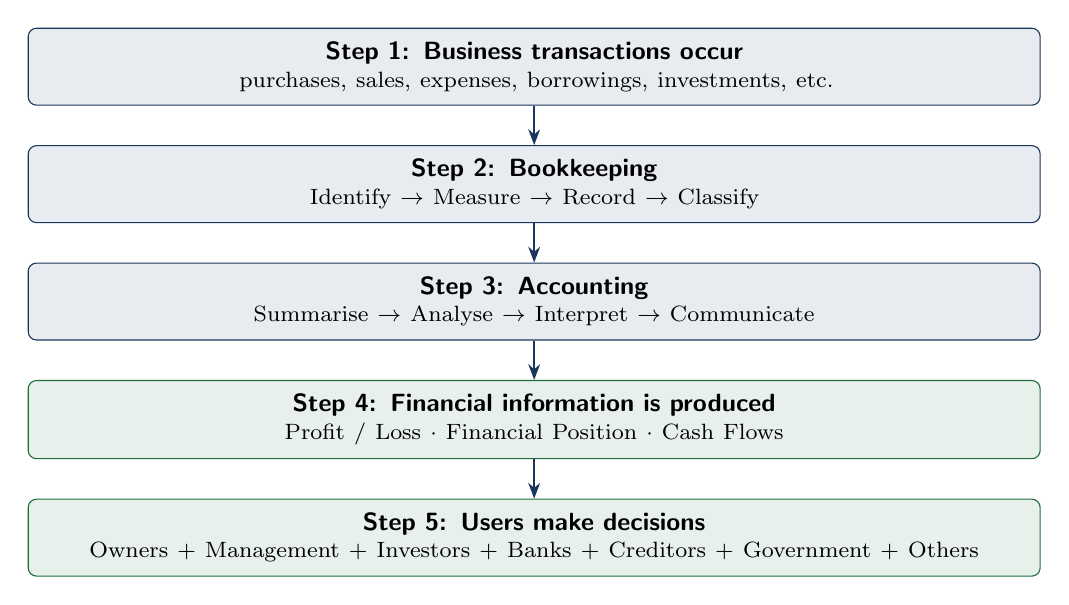
\begin{tikzpicture}[node distance=0.5cm]
  \node[flowbox,text width=12.5cm] (s1) {Step 1: Business transactions occur\\[-1pt]\normalfont\footnotesize purchases, sales, expenses, borrowings, investments, etc.};
  \node[flowbox,text width=12.5cm,below=of s1] (s2) {Step 2: Bookkeeping\\[-1pt]\normalfont\footnotesize Identify $\rightarrow$ Measure $\rightarrow$ Record $\rightarrow$ Classify};
  \node[flowbox,text width=12.5cm,below=of s2] (s3) {Step 3: Accounting\\[-1pt]\normalfont\footnotesize Summarise $\rightarrow$ Analyse $\rightarrow$ Interpret $\rightarrow$ Communicate};
  \node[outbox,text width=12.5cm,below=of s3] (s4) {Step 4: Financial information is produced\\[-1pt]\normalfont\footnotesize Profit / Loss $\cdot$ Financial Position $\cdot$ Cash Flows};
  \node[outbox,text width=12.5cm,below=of s4] (s5) {Step 5: Users make decisions\\[-1pt]\normalfont\footnotesize Owners $+$ Management $+$ Investors $+$ Banks $+$ Creditors $+$ Government $+$ Others};
  \foreach \x/\y in {s1/s2,s2/s3,s3/s4,s4/s5} \draw[arr] (\x) -- (\y);
\end{tikzpicture}
\end{center}

\subsection{Important conceptual connections}

\begin{center}
\small
\begin{tabularx}{\textwidth}{@{}l Y@{}}
\toprule
\rowcolor{acnavy!15}\textbf{Pair / group} & \textbf{Relationship}\\
\midrule
\textbf{Bookkeeping vs.\ accounting} & Bookkeeping $=$ recording and classification.\; Accounting $=$ summarising, analysis, interpretation and communication.\\
\textbf{Accountancy vs.\ accounting} & Accountancy $=$ the broader body of knowledge.\; Accounting $=$ the application or process of that knowledge.\\
\textbf{Financial accounting} & $\rightarrow$ Financial reporting\\
\textbf{Cost accounting} & $\rightarrow$ Cost determination and cost control\\
\textbf{Management accounting} & $\rightarrow$ Management planning, control and decisions\\
\bottomrule
\end{tabularx}
\end{center}

% =====================================================================
%                16. GLOSSARY
% =====================================================================
\section{Glossary of Key Terms}

\begin{center}
\small
\begin{tabularx}{\textwidth}{@{}l Y@{}}
\toprule
\rowcolor{acnavy!15}\textbf{Term} & \textbf{Meaning}\\
\midrule
\textbf{Accounting} & Process of identifying, recording, classifying, summarising, analysing, interpreting and communicating financial information\\
\textbf{Accountancy} & The systematic body of knowledge (principles, concepts, rules, conventions, techniques) behind accounting\\
\textbf{Bookkeeping} & Recording and classifying business transactions that have monetary aspects\\
\textbf{Business transaction} & A financially measurable economic event affecting the business\\
\textbf{Source document} & Evidence of a transaction: invoice, receipt, cash memo, bill, contract, bank document, purchase order\\
\textbf{Journal} & Book in which transactions are initially recorded, generally chronologically\\
\textbf{Subsidiary books} & Separate books of original entry for frequent transaction types\\
\textbf{Ledger} & Collection of individual accounts used to classify transactions account-wise\\
\textbf{Posting} & Transferring journal entries to the ledger accounts\\
\textbf{Trial balance} & Statement of ledger balances used mainly to check arithmetical equality of debits and credits\\
\textbf{Double entry} & Recording each transaction as equal debits and credits\\
\textbf{Financial statements} & Formal statements presenting performance, position and cash flows\\
\textbf{Income statement / P\&L} & Statement of profit or loss over a period\\
\textbf{Balance sheet} & Statement of assets, liabilities and equity at a date\\
\textbf{Cash flow statement} & Statement of cash inflows and outflows over a period\\
\textbf{Revenue} & Income earned from the business's activities\\
\textbf{Expense} & Cost incurred in earning revenue\\
\textbf{Profit} & Excess of revenue over expenses for a period\\
\textbf{Loss} & Excess of expenses over revenue for a period\\
\textbf{Assets} & Economic resources controlled by the business\\
\textbf{Liabilities} & Obligations of the business\\
\textbf{Equity / Capital} & Owners' residual interest in the business\\
\textbf{Receivables (debtors)} & Amounts owed to the business\\
\textbf{Payables (creditors)} & Amounts the business owes\\
\textbf{Inventory (stock)} & Goods held for sale (or for use in producing goods for sale)\\
\textbf{General Fund} & Net assets of a not-for-profit organisation\\
\textbf{Accounting period} & The span (month, quarter, year) for which results are determined\\
\textbf{Accounting cycle} & The repeated process by which transactions are recorded, processed and reflected in financial statements\\
\textbf{Window dressing} & Presenting accounts to look better than the actual condition\\
\textbf{Historical cost} & The original amount paid to acquire an asset\\
\bottomrule
\end{tabularx}
\end{center}

% =====================================================================
%                17. REVISION
% =====================================================================
\clearpage
\section{Revision}

\subsection{Quick revision sheet}

\begin{center}
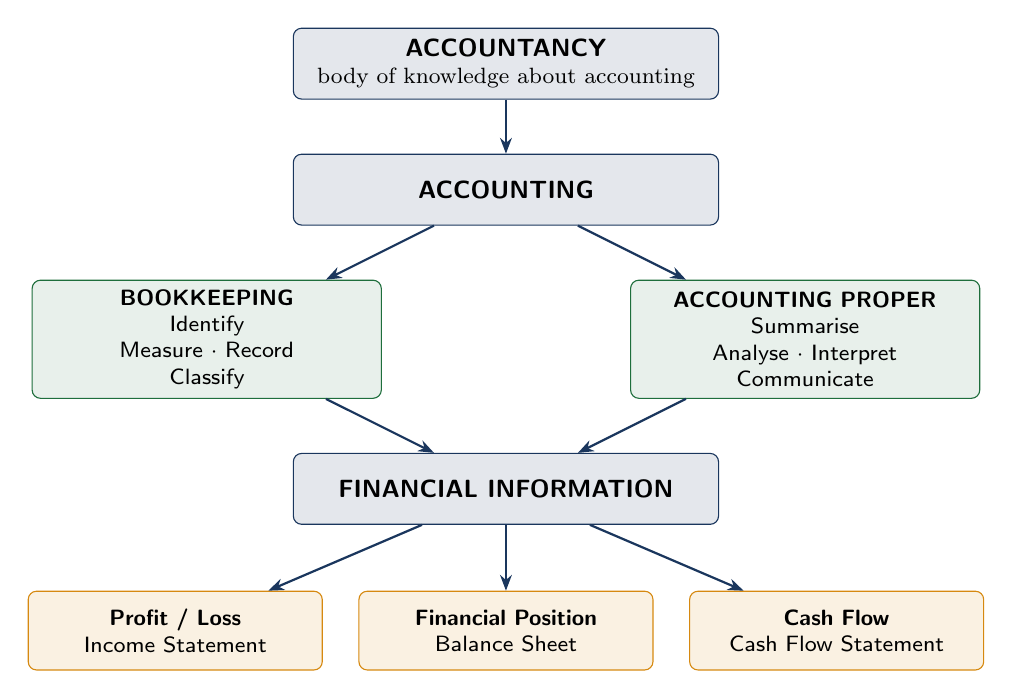
\begin{tikzpicture}[
  big/.style={draw=acnavy,fill=acnavy!12,rounded corners=3pt,align=center,font=\sffamily\small\bfseries,minimum width=5.4cm,minimum height=0.9cm},
  mid/.style={draw=acgreen,fill=acgreen!10,rounded corners=3pt,align=center,font=\sffamily\footnotesize,text width=4.2cm,minimum height=1.5cm},
  info/.style={draw=acamber,fill=acamber!12,rounded corners=3pt,align=center,font=\sffamily\footnotesize,text width=3.5cm,minimum height=1.0cm}]
  \node[big] (a) at (0,0) {ACCOUNTANCY\\[-1pt]\normalfont\footnotesize body of knowledge about accounting};
  \node[big] (b) at (0,-1.6) {ACCOUNTING};
  \node[mid] (c) at (-3.8,-3.5) {\textbf{BOOKKEEPING}\\Identify\\Measure $\cdot$ Record\\Classify};
  \node[mid] (d) at (3.8,-3.5) {\textbf{ACCOUNTING PROPER}\\Summarise\\Analyse $\cdot$ Interpret\\Communicate};
  \node[big] (e) at (0,-5.4) {FINANCIAL INFORMATION};
  \node[info] (f) at (-4.2,-7.2) {\textbf{Profit / Loss}\\Income Statement};
  \node[info] (g) at (0,-7.2) {\textbf{Financial Position}\\Balance Sheet};
  \node[info] (h) at (4.2,-7.2) {\textbf{Cash Flow}\\Cash Flow Statement};
  \draw[arr] (a) -- (b);
  \draw[arr] (b) -- (c);
  \draw[arr] (b) -- (d);
  \draw[arr] (c) -- (e);
  \draw[arr] (d) -- (e);
  \draw[arr] (e) -- (f);
  \draw[arr] (e) -- (g);
  \draw[arr] (e) -- (h);
\end{tikzpicture}
\end{center}

\subsection{Exam-oriented summary}

\begin{defbox}{Accounting (exam wording)}
Accounting is the process of \textbf{identifying, recording, classifying, summarising, analysing,
interpreting and communicating} financial information to users for \textbf{judgement and
decision-making}.
\end{defbox}

\begin{center}
\small
\begin{tabularx}{\textwidth}{@{}l Y@{}}
\toprule
\rowcolor{acnavy!15}\textbf{Topic} & \textbf{What to remember}\\
\midrule
\textbf{Seven functions} & I--R--C--S--A--I--C: Identify, Record, Classify, Summarise, Analyse, Interpret, Communicate\\
\textbf{Accounting cycle} & Transaction $\rightarrow$ Journal $\rightarrow$ Ledger $\rightarrow$ Trial Balance $\rightarrow$ Financial Statements (repeats each period)\\
\textbf{Accounting equation} & Assets $=$ Liabilities $+$ Equity\\
\textbf{Profit and loss} & Profit $=$ Revenue $-$ Expenses; Loss $=$ Expenses $-$ Revenue\\
\textbf{Double entry} & Total debits $=$ Total credits\\
\textbf{Father of Accounting} & Luca Pacioli, 1494, \emph{Summa de Arithmetica}, double-entry bookkeeping\\
\textbf{Four objectives} & Systematic records; profit or loss; financial position; information to interested parties\\
\textbf{Three branches} & Financial, cost, management accounting\\
\textbf{Science and art} & Science $=$ principles and knowledge; Art $=$ practical application\\
\textbf{Four limitations} & Qualitative factors, window dressing, historical cost, estimates and judgement\\
\textbf{Three information types} & Profit/loss (P\&L), position (Balance Sheet), cash flow (Cash Flow Statement)\\
\bottomrule
\end{tabularx}
\end{center}

\subsection{Common mix-ups}

\begin{impbox}[Traps to avoid]
\begin{itemize}
  \item \textbf{Accounting is not just bookkeeping.} Bookkeeping is one part of accounting
        (recording and classifying).
  \item \textbf{Profit is not cash.} A credit sale raises profit without raising cash.
  \item \textbf{A balanced trial balance is not proof of error-free books.}
  \item \textbf{Income statement is for a period; balance sheet is for a point in time.}
  \item \textbf{Window dressing is a misuse of accounting}, not a purpose of it.
  \item \textbf{Estimates are not arbitrary.} They follow principles, standards, evidence and
        professional judgement.
  \item \textbf{Pacioli documented and popularised} double entry; he did not invent bookkeeping from nothing.
  \item \textbf{Functions $\neq$ cycle.} Functions describe what accounting does; the cycle is the
        sequence of procedures.
\end{itemize}
\end{impbox}

\subsection{Central takeaway}

\begin{keybox}
A business generates financial transactions. Bookkeeping systematically records and classifies those
transactions. Accounting then summarises, analyses, interprets and communicates the resulting
information. This produces information about \textbf{profitability, financial position and cash
flows}, which users rely on for economic decision-making.
\end{keybox}

This foundation makes the upcoming topics much easier to connect: \textbf{accounting concepts and
principles, the accounting equation, debit--credit rules, journal entries, ledger, trial balance and
financial statements}. The course moves from \emph{what accounting is} to \emph{how individual
transactions actually affect accounts and financial statements}.

\subsection{Self-test questions}

\begin{enumerate}
  \item Define a business transaction and give one event that is \emph{not} an accounting transaction.
  \item Write the definition of accounting and list the seven functions in order.
  \item Which function answers ``Which transactions belong together?'' and through what is it carried out?
  \item State three differences between bookkeeping and accounting.
  \item List the five stages of the accounting cycle. Why is it called a cycle?
  \item Why does an agreeing trial balance not prove that the books are free from error?
  \item State the accounting equation. A business has assets of \Rs 3,00,000 and liabilities of
        \Rs 1,20,000. What is its equity?
  \item Distinguish between the income statement and the balance sheet on the basis of time perspective.
  \item A business makes a profit of \Rs 40,000 but its operating cash flow is negative. How is that possible?
  \item Name the three branches of accounting and state the main focus of each.
  \item Explain why accounting is both a science and an art.
  \item List and briefly explain the four limitations of accounting. Why is window dressing not a purpose of accounting?
  \item Who is the Father of Accounting and why?
\end{enumerate}

\subsection{Answer key}

\begin{enumerate}
  \item A measurable economic event with a financial effect on the business (e.g.\ paying rent). A
        decision to hire an employee next month is not yet a transaction.
  \item See the definition in Section~2; Identify, Record, Classify, Summarise, Analyse, Interpret, Communicate.
  \item Classifying, through ledger accounts.
  \item E.g.\ objective (record vs.\ ascertain results and position), stage (primary vs.\ secondary), skills
        (clerical vs.\ analytical), and who performs it (bookkeepers vs.\ accountants).
  \item Transaction, journal, ledger, trial balance, financial statements. The process repeats every accounting period.
  \item Errors such as omitted transactions, wrong-account postings or offsetting errors leave debit and credit totals equal.
  \item Assets $=$ Liabilities $+$ Equity. Equity $=3{,}00{,}000-1{,}20{,}000=\Rs\,1{,}80{,}000$.
  \item The income statement covers a period of time; the balance sheet is a snapshot at a point in time.
  \item Credit sales: revenue is recognised, so profit arises, but cash has not yet been received (see the case study in Section~9).
  \item Financial accounting (reporting), cost accounting (cost determination and control), management
        accounting (planning, control and decisions).
  \item Science: systematic body of principles and standards. Art: practical application of those principles.
  \item Qualitative factors ignored; window dressing; historical cost; estimates and judgement. Window dressing is a misuse or
        manipulation of information, not an aim of accounting.
  \item Luca Pacioli, who documented and popularised double-entry bookkeeping in 1494.
\end{enumerate}

\end{document}
